%
% PKUMpLtX --- A LaTeX document class for 'Modern Physics Laboratory' in PKU based on `revtex4-2`
%
% Please read `README.md' and the template file before using
% 需要确保 font 选项指定的字体已安装! 具体参见 `README.md' 的说明.
\documentclass[font=default]{mpltx}

% 以下至 \begin{document} 都仅是本文件为了方便额外定义的命令, 写报告时不需要.
\hypersetup{colorlinks=true}% 超链接带颜色
\usepackage{xcolor}
\newcommand{\note}[1]{{\color{gray}#1}}
\NewDocumentCommand{\pkg}{s o m}{%
    \IfBooleanF{#1}{%
        \IfNoValueTF{#2}%
            {\href{https://www.ctan.org/pkg/#3}}%
            {\href{https://www.ctan.org/pkg/#2}}%
    }%
    {\textsf{#3}}%
}
\newcommand*\cs[1]{\texttt{\textbackslash #1}}
\newcommand*\env[1]{\textit{\texttt{#1}}}
\newcommand*\code[1]{\texttt{#1}}
\newcommand*\file[1]{\textbf{\texttt{#1}}}
\makeatletter
\newcommand\releasedate{%
    \href{https://github.com/CastleStar14654/PKUMpLtX/releases/tag/\mpltx@fileversion}%
        {\mpltx@filedate, \mpltx@fileversion}}
\makeatother
% 以上是本文件为了方便额外定义的命令, 写报告时不需要.

\begin{document}

\title{非线性对流斑图实验报告} % 切合报告内容, 简短明确, 可以不同于讲义
\author{李钰欣} % 这里 \emailphone 一定要紧跟在 \author 后方
\emailphone{2300011368@stu.pku.edu.cn}{(86)15816647600}
% 如果改用 \email 则仅需要邮箱参数
\affiliation{北京大学物理学院\quad 学号: 2300011368}
% % 可以使用 \zhdate 自动生成中文日期, 如
\date{\zhdate{2025/10/16}}
% % 也可使用 babel 的 \localedate, 如
% \date{\localedate{2020}{12}{1}}
% % 两者均会输出 `2020 年 12 月 1 日'
% 下面的 \date 的参数是为了自动输出正确版本号, 正式报告请替换为上面的两种 \date 之一
% \date{\releasedate}
\begin{abstract}
本实验通过设置电流调整上下表面温差,并利用阴影法,得到不同温差、不同流体厚度下的对流斑图。
通过本实验,对对流现象有了更深入的认识,也对耗散结构理论有了初步的了解。

\end{abstract}
\keywords{非线性热对流,耗散结构}

\maketitle

\section{引言}

因热力作用使得流体状态(密度、压力等)发生差异可以引起流体运动,称为热对流。
对具有自由面-固壁底层的流体薄层进行底层加热,可以观察到各种对流图形,称为斑图。
本实验观测非线性热对流斑图,从而对耗散结构理论有一个初步的认识。

 
\section{理论}\label{sec:theory}
由NS方程、流体连续性方程、热传导方程,并假定存在微扰$T = T_0(z) + \theta$,$p = p_0(z) + p'$,$\mathbf{V} = \mathbf{u}$,
代入方程组并作去量纲化可以得到:

$$
\begin{cases}
\sigma^{-1} (\frac{\partial u}{\partial t} + \mathbf{u} \cdot \nabla \mathbf{u}) = \theta z - \nabla \mathbf{p} + \nabla^2 \mathbf{u} \\
\nabla \cdot \mathbf{u} = 0 \\
\frac{\partial \theta}{\partial t} + \mathbf{u} \cdot \nabla \theta = Ra \omega + \nabla^2 \theta
\end{cases}
$$

其中边界条件为$\theta = u = 0$, $z = \pm \frac{1}{2}$,$Ra \equiv \frac{g \alpha d^3 \Delta T}{\kappa \gamma}$
被称为瑞利数。

通过数值计算结果显示有临界参量:$R_c = 1707.76, q_c = 3.117$,也就是说,当对流水层的上下温差使得瑞利数Ra<$R_c$时,系统保持定态解稳定;
当Ra>$R_c$时,满足条件的部分扰动噪声就会逐渐变大,大到一定程度时,方程中的非线性项就不能忽略,进而得到的解可以理解实验结果的斑图分叉行为。


\section{实验装置}
实验装置示意图:见图1

\begin{figure}
  \centering
  \includegraphics[width=0.85\linewidth]{fig/instrument3.jpg}
  \caption{非线性对流斑图实验装置示意图}
  \label{sec:instrument3}
\end{figure}

主要装置:

小薄层的对流水层,其上为降温水层,两个水层间为蓝宝石片(热导率46W/m $\cdot$ K);对流水层下表面是黄金镀黄铜盘,利用硅胶片通电加热保持其温度均匀性。

实验装置中光路部分得到准平行光光束,进而通过阴影法得到斑图。

\section{结果及讨论}
1.实验数据
水层为2mm时:

\begin{table}[!ht]
    \centering
    \begin{tabular}{|l|l|l|l|}
    \hline
电流(mA)         & 下层温度(摄氏度)         &上层温度(摄氏度)        &温差(摄氏度)         \\  \hline
0                     & 24.4                      &26.1              &-1.7 \\ \hline
500                    & 26.9                      &26.9             &0      \\ \hline
850                     & 32.3                     &28.7              &3.6      \\ \hline
900                     & 34.7                    &29.8               &4.9  \\ \hline
950                      &36.3                     &30.9            & 5.4   \\ \hline
1000                     & 37.9                    &31.9              &6       \\ \hline
1200                    & 42.3                     &34.0              &8.3      \\ \hline
    \end{tabular}
\end{table}

水层为4mm时:

\begin{table}[!ht]
    \centering
    \begin{tabular}{|l|l|l|l|}
    \hline
电流(mA)         & 下层温度(摄氏度)       &上层温度(摄氏度)     &温差(摄氏度)         \\  \hline
0                     & 27.6                      &29.7              &-2.1     \\ \hline
200                    & 27.3                      &29.3             &-2       \\ \hline
400                     & 28.8                    &29.3              &-0.5     \\ \hline
600                     & 31.1                    &29.4              &1.7      \\ \hline
900                      &36.2                     &30.3            & 5.9      \\ \hline
1200                     & 43.6                    &32.0              &11.6    \\ \hline
1500                    & 42.3                     &34.0              &8.3     \\ \hline
    \end{tabular}
\end{table}

2.现象及分析
水层为2mm时,在电流950mA之前显示均匀圆光斑,在电流950mA(温差5.4摄氏度)时出现同心圆斑图,如图2所示。此后斑图逐渐明显。

\begin{figure}
  \centering
  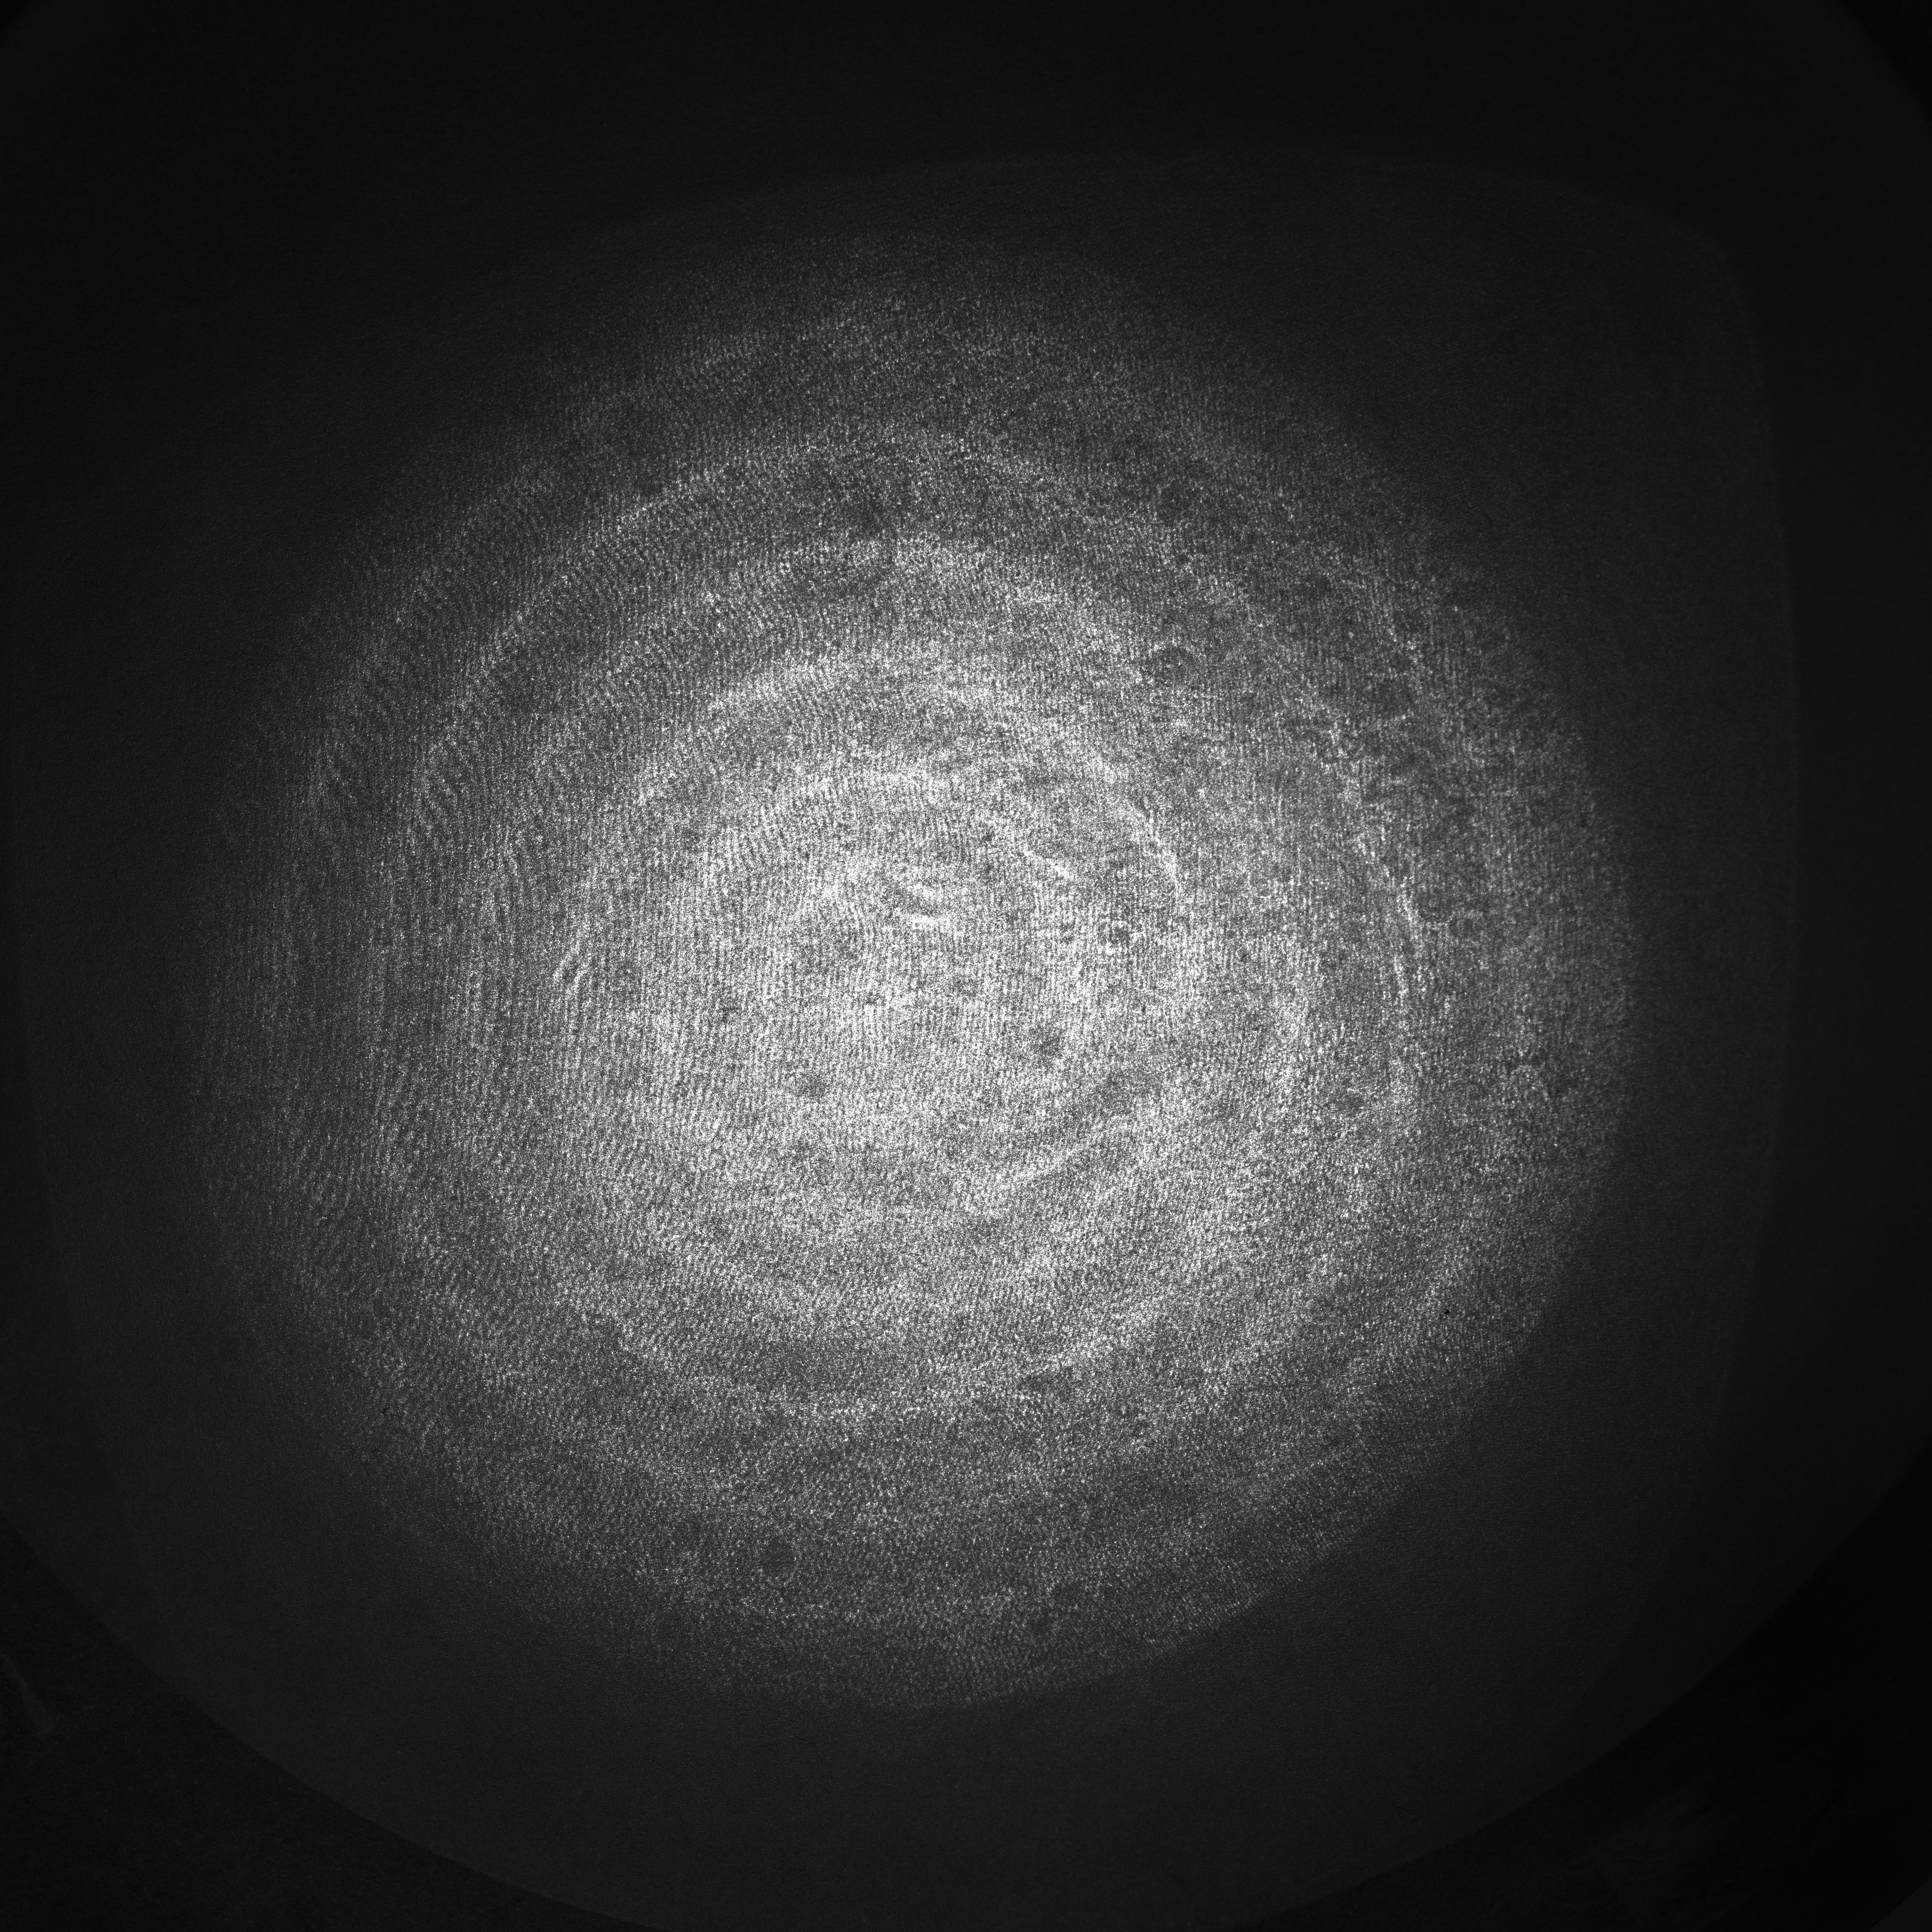
\includegraphics[width=0.85\linewidth]{fig/num1.jpg}
  \caption{2mm 950mA时的斑图}
  \label{sec:num1}
\end{figure}

水层为4mm时,在电流600mA前无明显现象,600mA(温差1.7摄氏度)时隐约出现同心圆,如图3所示。
此后随电流增大即温差升高,同心圆逐渐扭曲并出现分支结构,如图4所示。

\begin{figure}
  \centering
  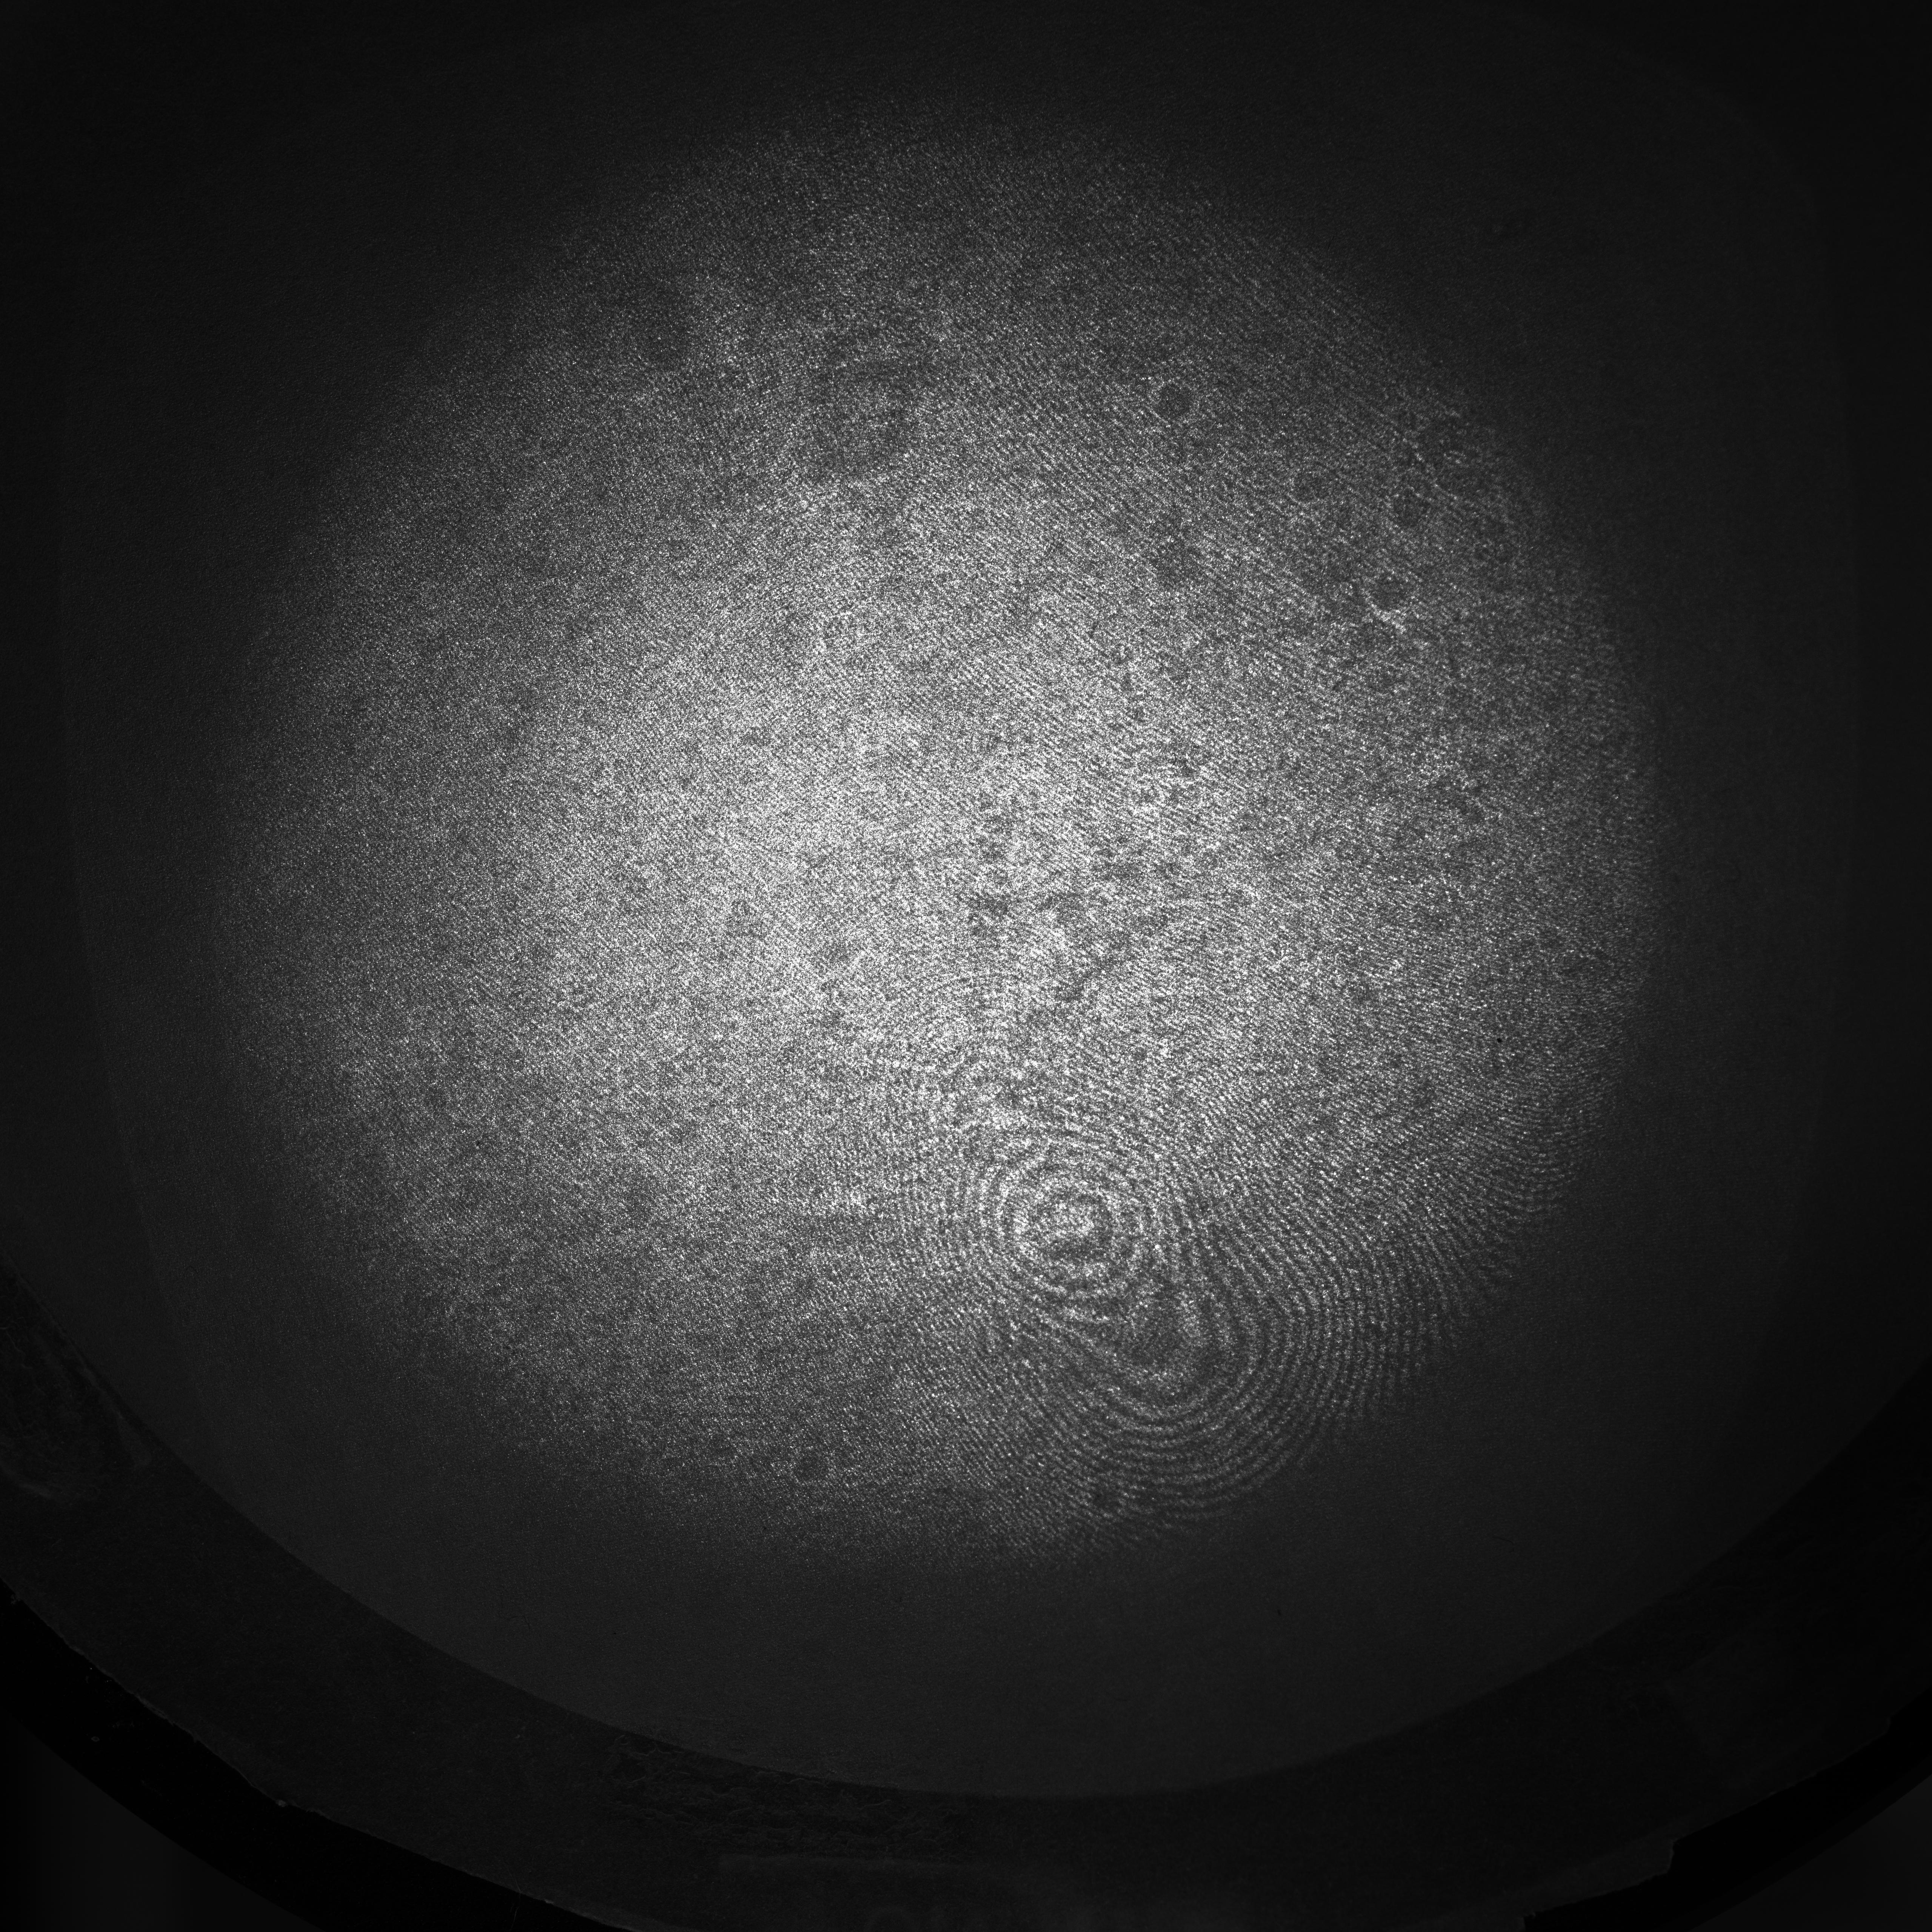
\includegraphics[width=0.85\linewidth]{fig/num2.jpg}
  \caption{4mm 600mA时的斑图}
  \label{sec:num2}
\end{figure}


\begin{figure}
  \centering
  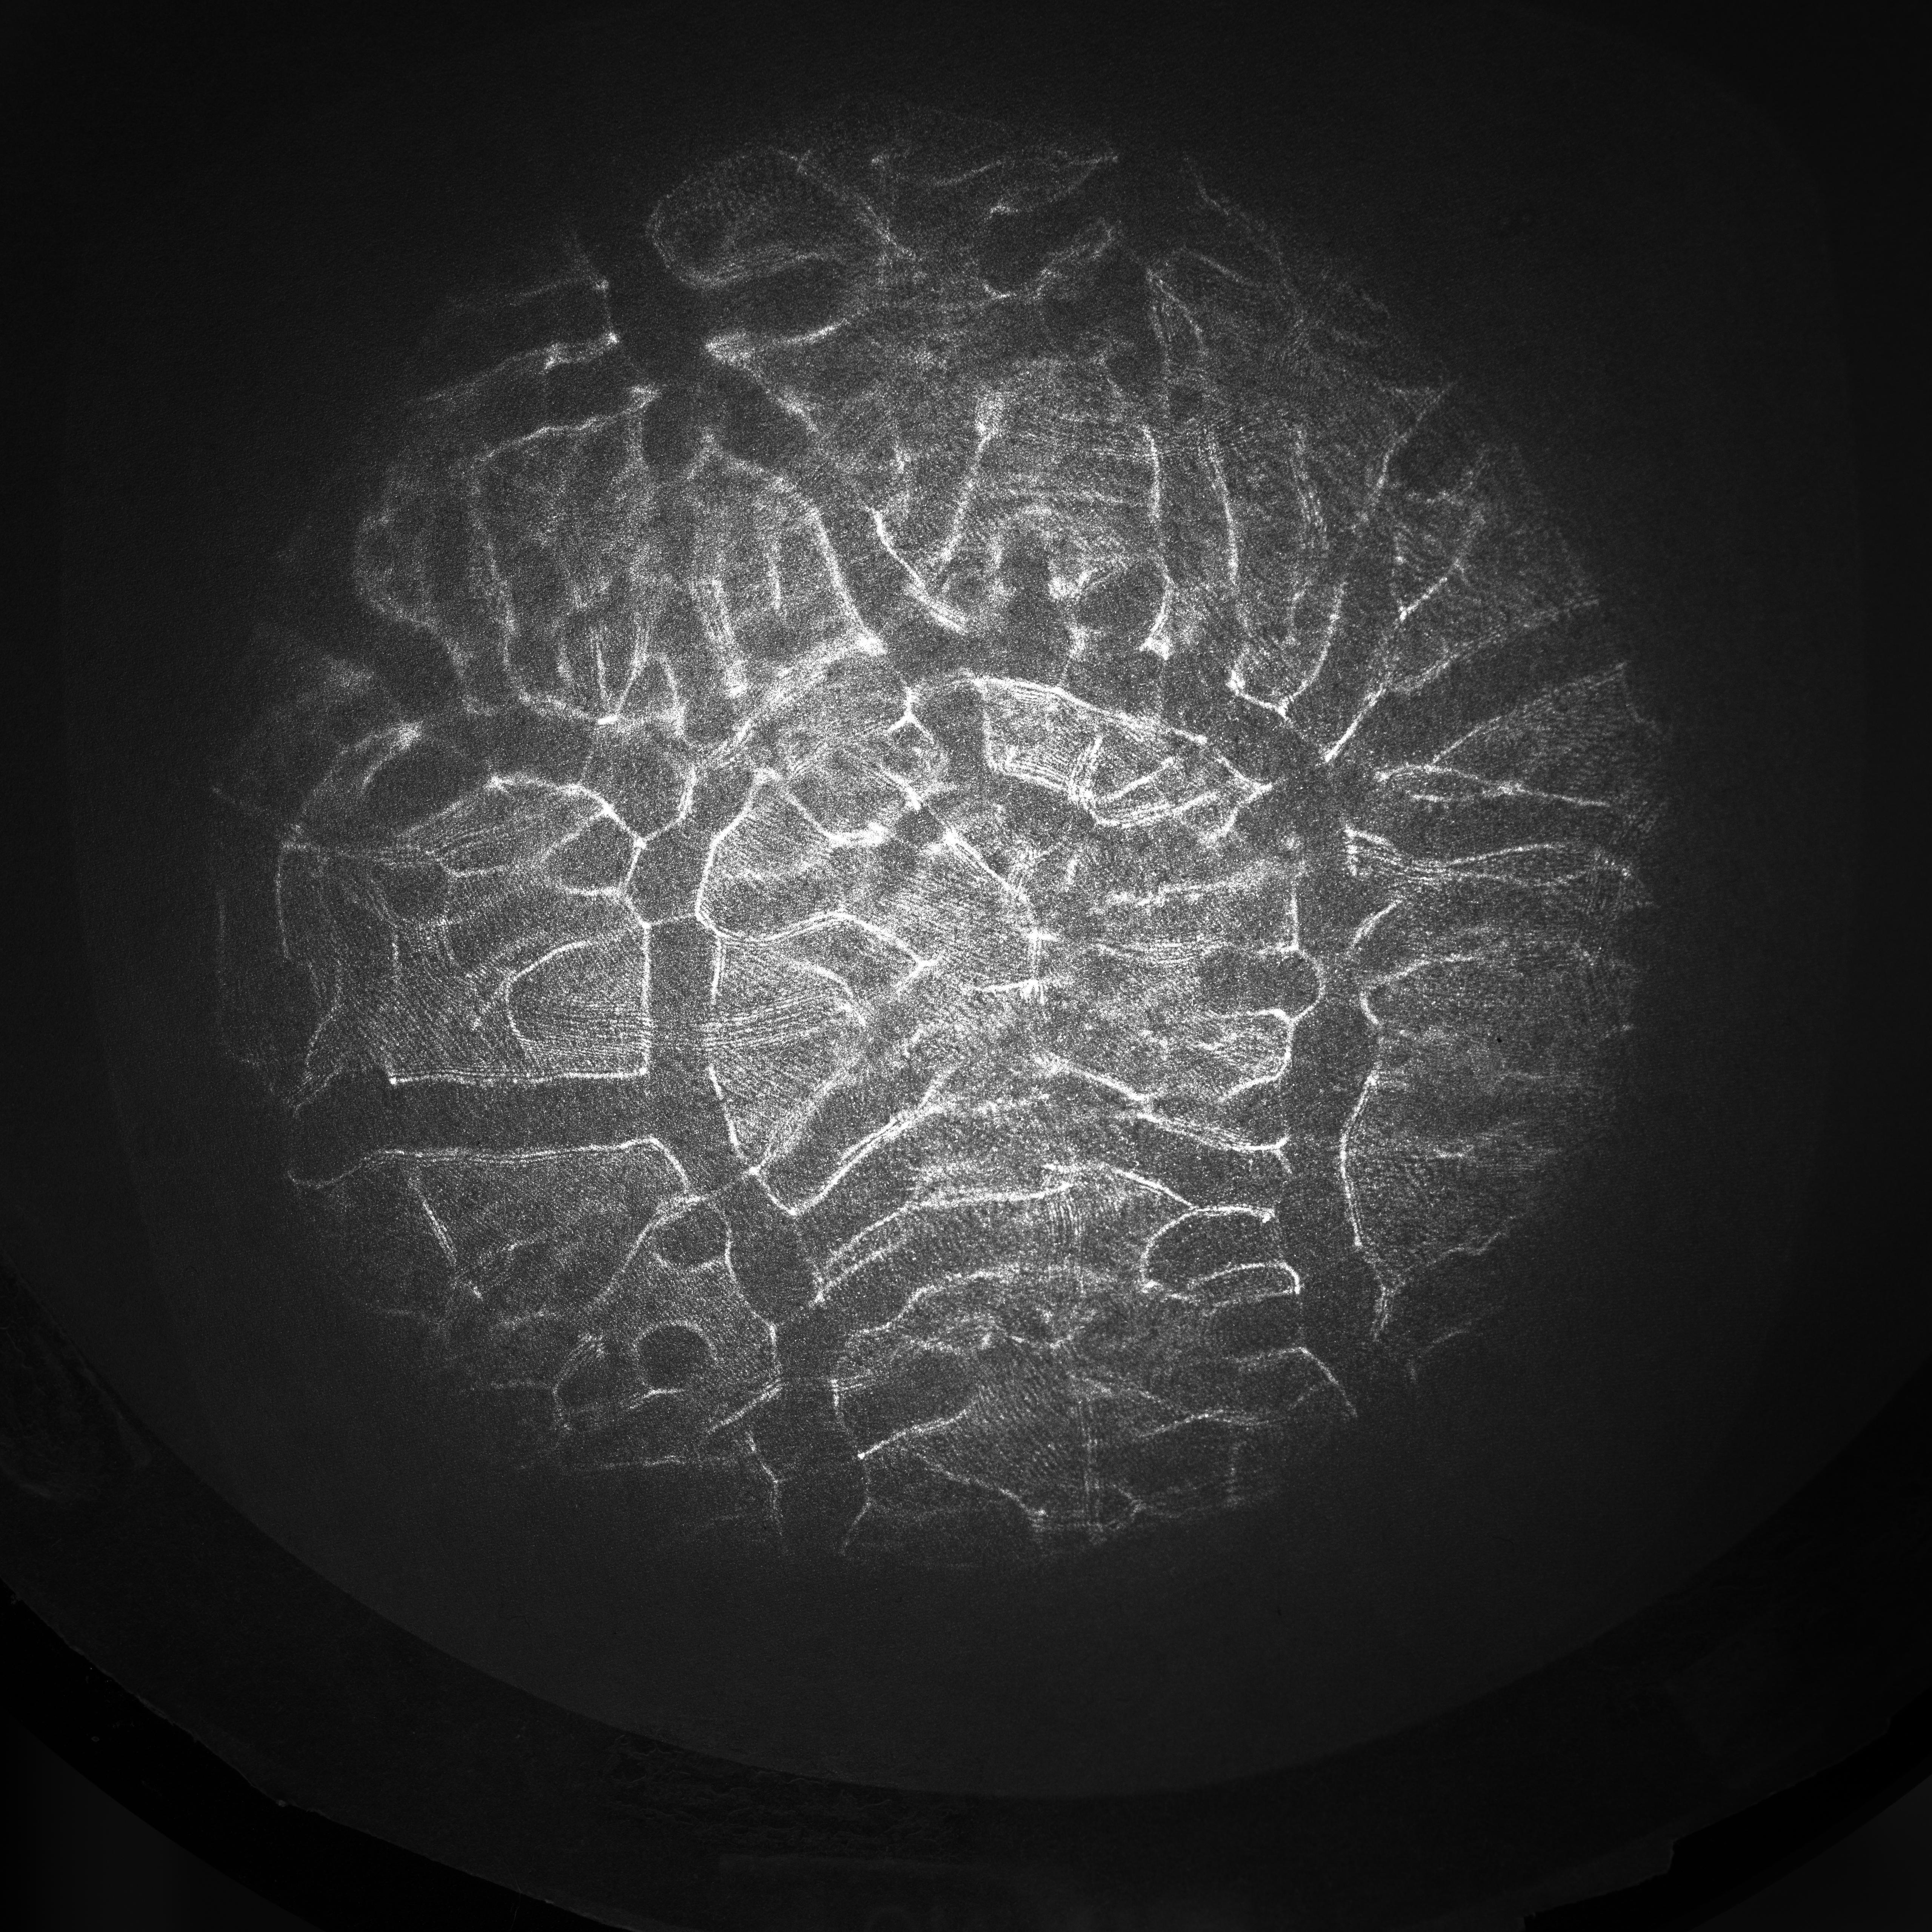
\includegraphics[width=0.85\linewidth]{fig/num3.jpg}
  \caption{4mm 1500mA时的斑图}
  \label{sec:num3}
\end{figure}


由于随着温度变高,水层密度变小,折射率变小,故可以类比冷水为凸透镜,亮线对应冷水即由上往下流动的水。
每两个亮线之间存在两个热流圆包。

当水层换成4mm时,由$Ra \equiv \frac{g \alpha d^3 \Delta T}{\kappa \gamma}$可知临界温度变小。理论上临界温度应当为原来的八分之一,
实际上约为三分之一,原因有:一,实际实验中侧面散热更大;二,临界时振幅为0,观测到斑图时已经不在临界点,实验误差较大。

用特征波长代表斑图的空间特征尺度,临界状态下特征波长约等于谁层厚度的两倍,也就是说斑图的空间特征尺度与水层厚度有线性关系。

本实验时耗散结构理论的一个证明。耗散结构理论是指,一个远离平衡的开放系统,当描述系统离开平衡态的参量达到一定阈值,系统会出现分叉行为,
在越过分叉点后,系统将离开原来无序的热力学分支,发生突变进入一个全新的稳定有序状态。本实验在水层到达平衡态后在上下表面施加温度差,
随着温度差提升而显示规则的同心圆斑图,例证了耗散结构理论。


\section{结论}
本实验通过设置电流调整上下表面温差,并利用阴影法,得到不同温差、不同流体厚度下的对流斑图,并获得了2mm和4mm时对应的临界温度。
通过本实验,对对流现象有了更深入的认识,也对耗散结构理论有了初步的了解。

\end{document}





